\documentclass[journal = jacsat, manuscript = suppinfo]{achemso}

\usepackage[version = 4]{mhchem}
\usepackage{graphicx}
\usepackage{mwe}
\usepackage{textcomp}
\usepackage{gensymb}
\usepackage{booktabs}

% disable symbol next to email
\makeatletter
\def\acs@author@fnsymbol#1{}
\makeatother
% enable TOC
\SectionNumbersOn

% macros
\newcommand{\h}{$^1$H}
\newcommand{\p}{$^{31}$P}
\newcommand{\cdcl}{\ce{CDCl3}}
\newcommand{\del}{$\delta = $}
\newcommand{\wavenum}{cm$^{-1}$}
\newcommand{\kmn}{\ce{KMnO4}}
\newcommand{\chcl}{\ce{CHCl3}}
\newcommand{\acac}[1]{\ce{#1(acac)3}}
\newcommand{\acactwo}[1]{\ce{#1(acac)2}}

\title{Identification of Unknown Metal Acetylacetonate Complexes via Evan's Method}

\author{David Qiu}
\affiliation{Department of Chemistry, University of Illinois at
Urbana-Champaign, 505 S Matthews Avenue, Urbana, IL, 61801}
\email{davidlq2@illinois.edu}

\begin{document}

\tableofcontents

\newpage

\section{General Considerations}

\kmn, acetylacetonate, \cdcl, and \chcl\ were all sourced from Oakwood
Chemicals. A Bruker U500 500 MHz NMR spectrometer was used to obtain all \h\ NMR
spectra.

\section{Experimental}

\subsection{Synthesis of \acac{Mn} \cite{handout, textbook}}

To a 250 mL beaker was charged 0.500 g \kmn\ (3.16 mmol, 1 equiv.), 75 mL DI
water, and a stir bar. This solution was heated to 70 \degree C with stirring
until total dissolution. The beaker was cooled in an ice bath, and 2.30 mL
acetylacetone (22.4 mmol, 7 equiv.) was slowly poured in over the course of 3
minutes. The solution was brought to a boil for 5 minutes, and was cooled again
in an ice bath. The dark brown \acac{Mn} crystals were then filtered through a
coarse glass frit, washed with 10 mL DI water 3 times, and dried on vacuum for
30 minutes. This reaction resulted in a percent yield of 41\% (0.46 g total,
1.11 g exp.).

\subsection{Measurement of Magnetic Moments \cite{handout}}

A capillary tube containing 2 mL of 50:1 (v/v) deutero:proteo chloroform was
inserted into a NMR tube. NMR samples were prepared through the addition of
10--15 mg of the species and 600 \micro L of the same chloroform solution. This
procedure was performed for \acac{Mn} and the four unknown samples provided.  A
summary of observations for each of the unknowns is tabulated below.  The colors
of the unknowns agree well with the colors of their assignments in literature.
\cite{cracac_color, feacac_color, textbook_2}

\tabcolsep=0.11cm
\begin{table}
\begin{tabular}{clcccccl}
\toprule
Unk.\ No.\ &           Color &  $m_\text{solid}$ (g) &  $m_\text{solvent}$ (g) &  $\Delta\nu$ (Hz) &   T (K) & $\mu$ ($\mu_\text{B}$) & Assignment\\
\midrule
\acac{Mn} & Purple &    0.0149 &         0.977 &    1315 &  293 & 4.97 & -- \\
1 &        Green &      0.0226 &         1.240 &       0 &  293 & 0    & Low-spin \acac{Co} \\
2 &       Violet &      0.0158 &         0.625 &     635 &  293 & 2.57 & \acac{Cr} \\
3 &      Crimson &      0.0154 &         0.306 &    1700 &  293 & 2.97 & High-spin\acac{Fe}  \\
4 &    Blue-Gray &      0.0156 &         0.885 &     345 &  293 & 1.96 & \acactwo{Cu} \\
\bottomrule
\caption{Table of observations recorded for each of the unknowns.}
\end{tabular}
\end{table}

All spectra were baselined, phase-corrected, and referenced according to the
control TMS peak (identified by its lack of peak broadening) prior to analysis.
The ``p" prefix denotes the paramagnetically shifted peak. The \h\ NMR
interpretation (500 MHz, $\delta$, 50:1 d:p chloroform) is as follows.
\textbf{\acac{Mn}:} 7.32 ppm (\chcl), 4.70 ppm (p-\chcl), 2.17 ppm (\acac{Mn}).
\textbf{Unknown 1:} 7.27 ppm (\chcl).
\textbf{Unknown 2:} 7.26 ppm (\chcl), 8.53 ppm (p-\chcl).
\textbf{Unknown 3:} 7.26 ppm (\chcl), 10.66 ppm (p-\chcl).
\textbf{Unknown 4:} 7.26 ppm (\chcl), 7.96 ppm (p-\chcl).
The lineshape of paramagnetically shifted peaks were observed to be heavily
broadened, in excellent agreement with existing \h\ NMR spectra of paramagnetic
compounds. \cite{paramag_nmr}

\section{\h\ NMR Spectra}

In each of the following NMR spectra, there exists instrumental artifact
immediately upfield each peak, altering their peak shape. These are not
paramagnetic shifts, nor are they impurities. They are labelled with an asterisk
``*".

\subsection{\h\ NMR Spectra of \acac{Mn}}

\begin{figure}[H]
	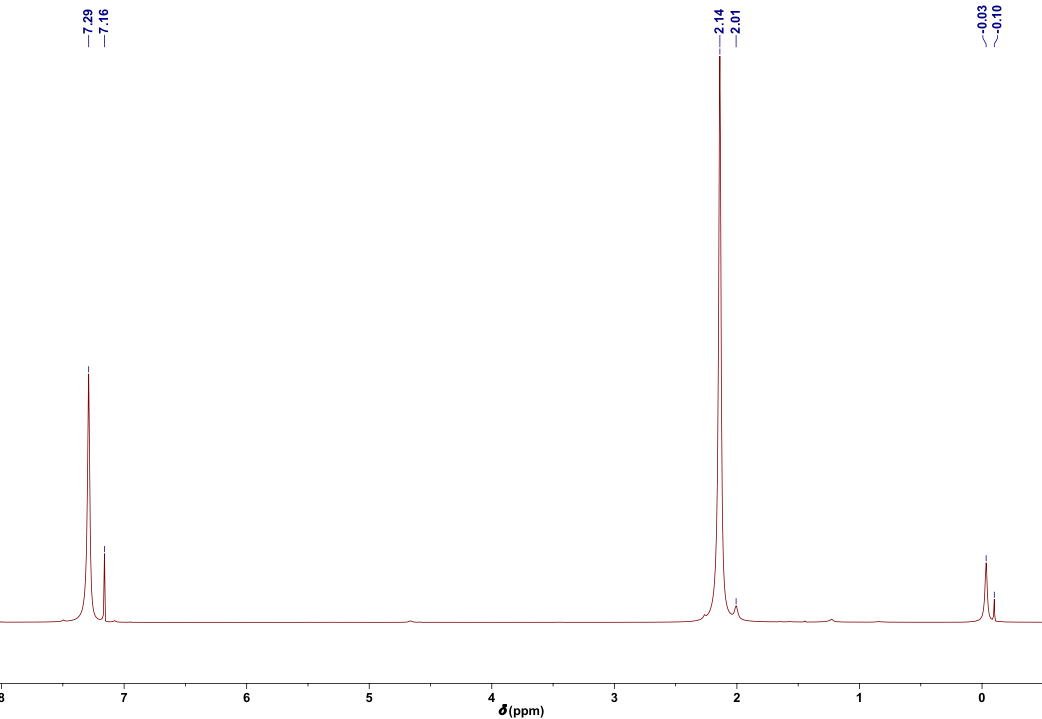
\includegraphics[width=\textwidth]{figures/mnacac_hnmr.png}
	\caption{Fully interpreted \h\ NMR spectrum of \acac{Mn}. Observe the
	instrument artifact immediately upfield each peak.}
\end{figure}

\begin{figure}[H]
	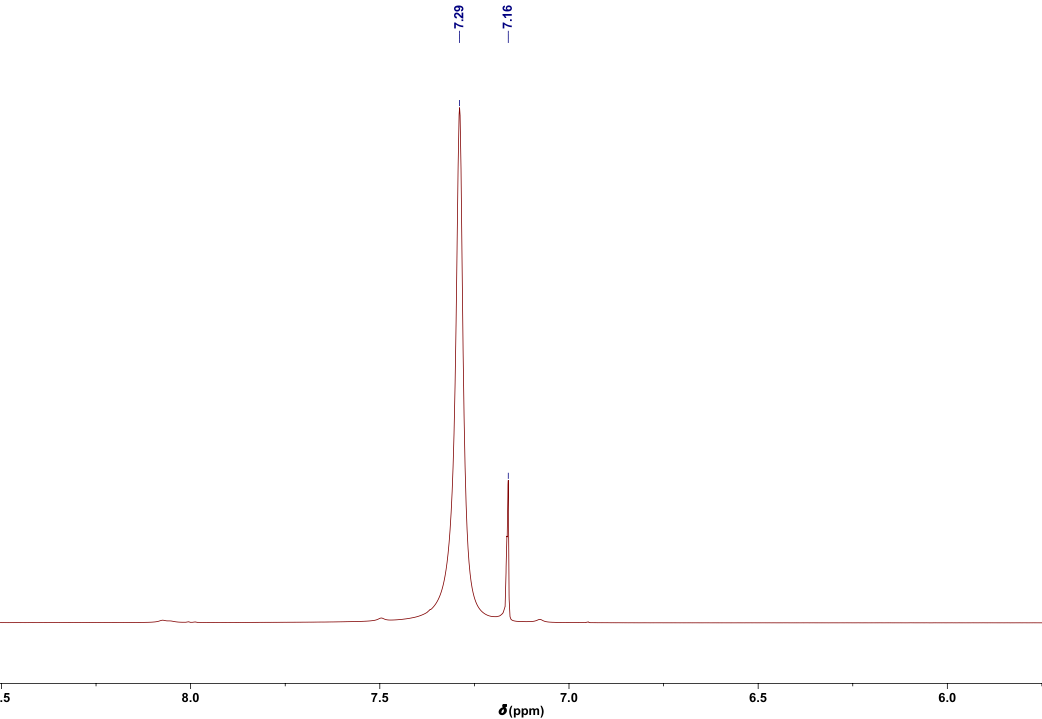
\includegraphics[width=\textwidth]{figures/mnacac_zoom_hnmr.png}
	\caption{\h\ NMR spectrum of \acac{Mn}, highlighting the assigned \chcl\
	and p-\chcl\ peaks.}
\end{figure}

\subsection{\h\ NMR Spectrum of Unknown 1}

\begin{figure}[H]
	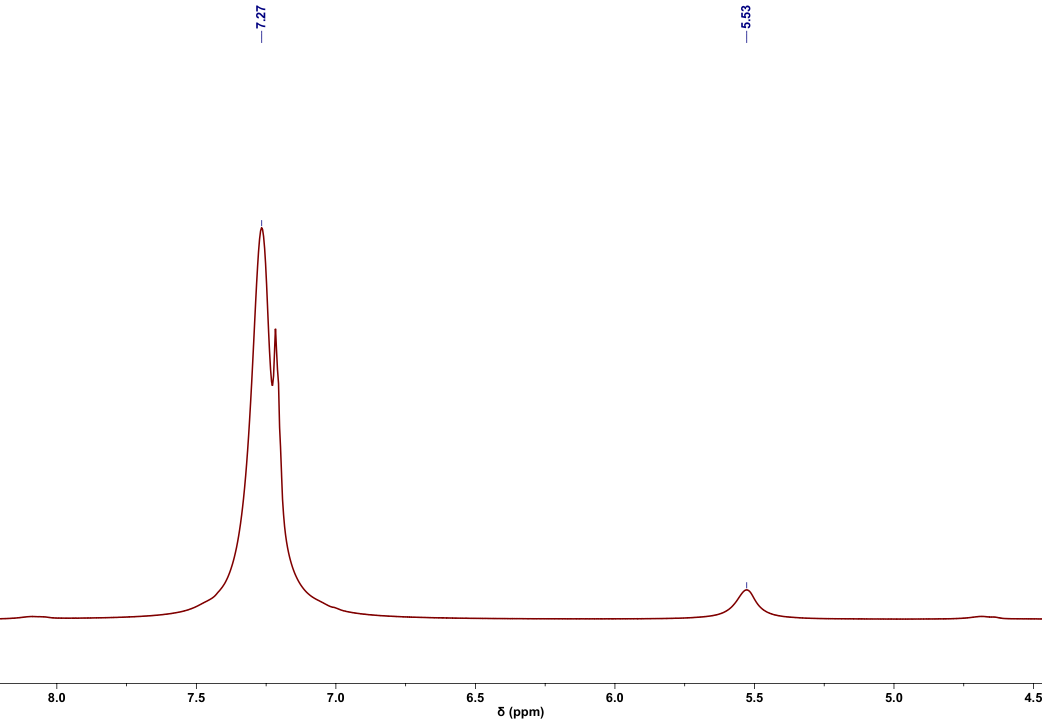
\includegraphics[width=\textwidth]{figures/unk1_hnmr.png}
	\caption{\h\ NMR spectrum of Unknown 1, highlighting the assigned \chcl\
	and p-\chcl\ peaks. The peak at 5.53 ppm is an instrumental artifact
	found upfield each peak in the full \h\ NMR spectrum (not shown).}
\end{figure}

\subsection{\h\ NMR Spectrum of Unknown 2}

\begin{figure}[H]
	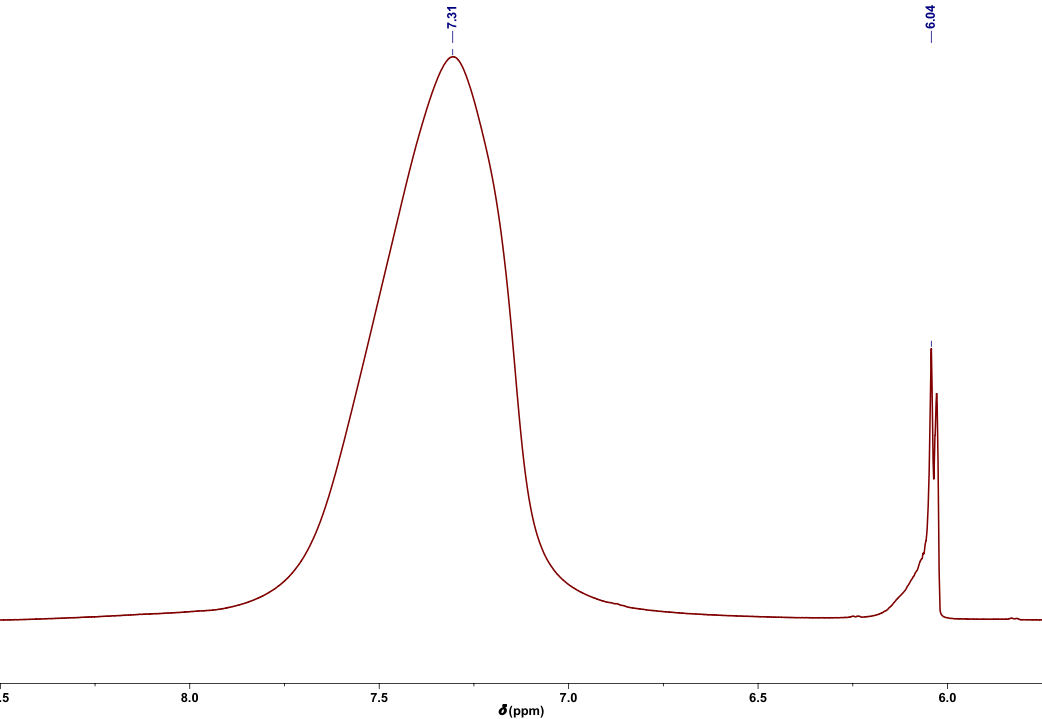
\includegraphics[width=\textwidth]{figures/unk2_hnmr.png}
	\caption{\h\ NMR spectrum of Unknown 2, highlighting the assigned \chcl\
	and p-\chcl\ peaks.}
\end{figure}

\subsection{\h\ NMR Spectrum of Unknown 3}

\begin{figure}[H]
	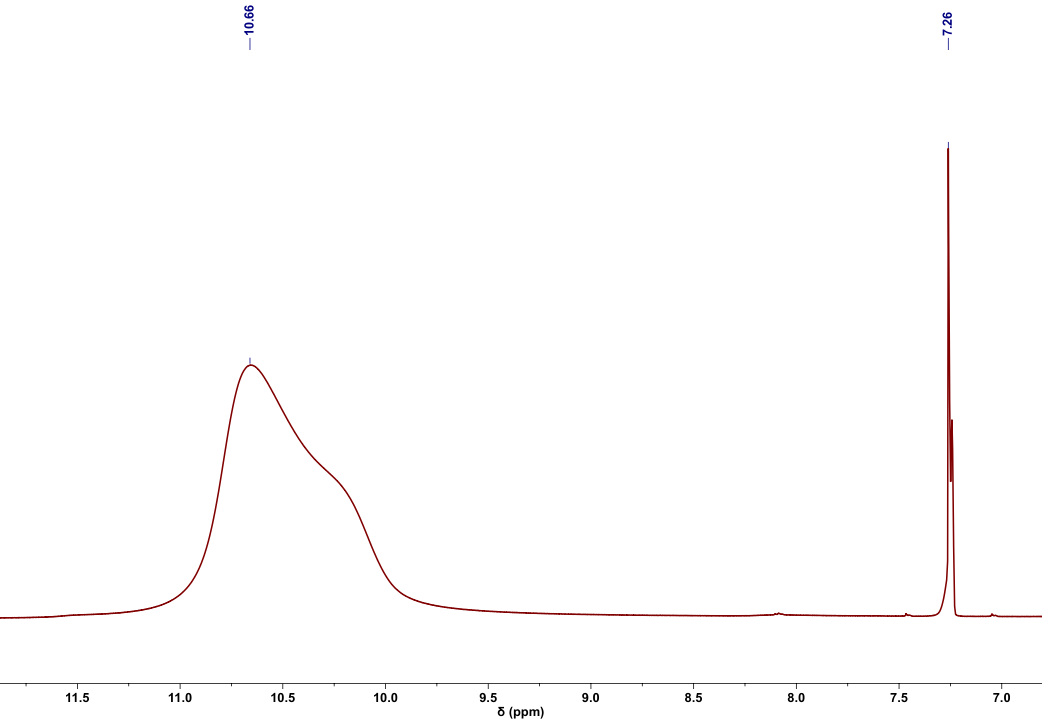
\includegraphics[width=\textwidth]{figures/unk3_hnmr.png}
	\caption{\h\ NMR spectrum of Unknown 3, highlighting the assigned \chcl\
	and p-\chcl\ peaks.}
\end{figure}

\subsection{\h\ NMR Spectrum of Unknown 4}

\begin{figure}[H]
	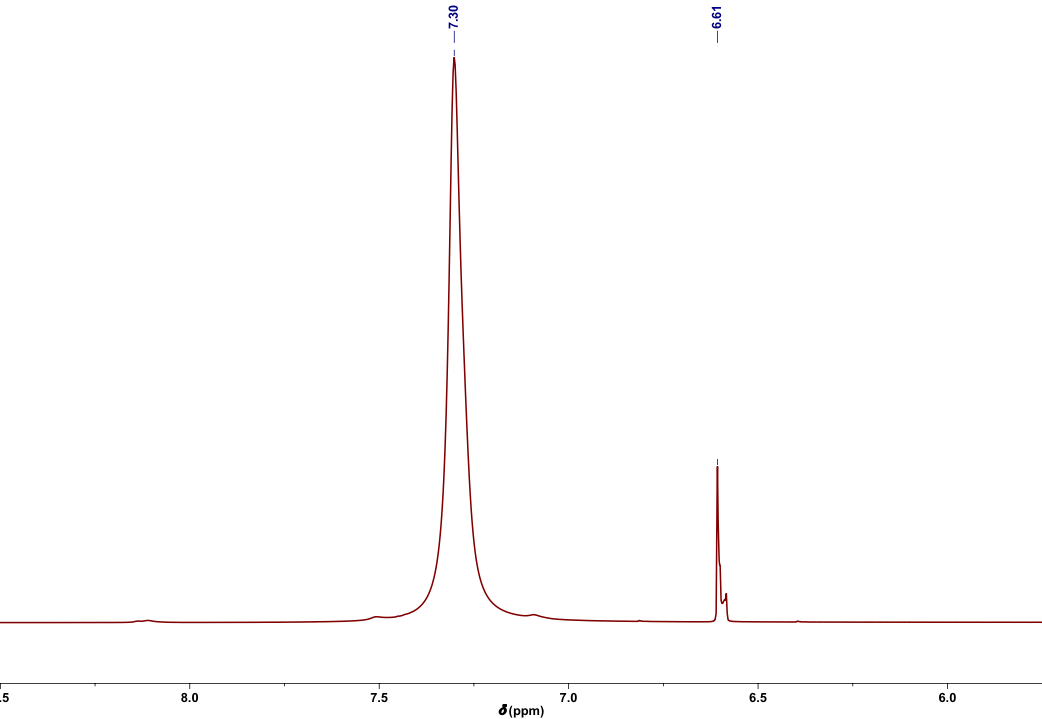
\includegraphics[width=\textwidth]{figures/unk4_hnmr.png}
	\caption{\h\ NMR spectrum of Unknown 4, highlighting the assigned \chcl\
	and p-\chcl\ peaks.}
\end{figure}

\section{Magnetic Moment Data}

Unknowns were determined by computing the absolute difference with respect to
the magnetic moments of the low and high-spin complexes of interest. The full
set of data is tabulated below. Unknown 1 is excluded from Tables S3 and S4 on
the basis of being diamagnetic.

\subsection{Tabulated Values of $\mu$}

\begin{table}[H]
\begin{tabular}{lcccccccc}
\toprule
Sample &        Ti &         V &        Cr &        Mn &        Fe &        Co &        Ni &        Cu \\
\midrule
Mn(acac)3 &  4.72 &  4.75 &  4.75 &  4.77 &  4.78 &  4.80 &  4.80 &  4.83 \\
Unknown 1 &  0    &  0    &  0    &  0    &  0    &  0    &  0    &  0    \\
Unknown 2 &  2.55 &  2.56 &  2.56 &  2.57 &  2.58 &  2.59 &  2.59 &  2.61 \\
Unknown 3 &  2.96 &  2.97 &  2.97 &  2.99 &  2.99 &  3.00 &  3.00 &  3.02 \\
Unknown 4 &  1.90 &  1.91 &  1.91 &  1.92 &  1.93 &  1.94 &  1.94 &  1.96 \\
\bottomrule
\end{tabular}
\caption{$\mu$ for each of the samples in units of $\mu_\text{B}$, calculated
given the molar masses of the elements listed in the columns.}
\end{table}

\subsection{Tabulated Values of $|\Delta\mu|$ for High-Spin Complexes}

\begin{table}[H]
\begin{tabular}{lcccccccc}
\toprule
Sample &        Ti &         V &        Cr &        Mn &        Fe &        Co &        Ni &        Cu \\
\midrule
Mn(acac)3 &  2.99 &  1.92 &  0.88 &  0.12 &  1.13 &  0.09 &  0.93 &  2.00 \\
Unknown 2 &  0.82 &  0.26 &  1.30 &  2.32 &  3.33 &  2.30 &  1.27 &  0.21 \\
Unknown 3 &  1.23 &  0.14 &  0.89 &  1.90 &  2.92 &  1.89 &  0.86 &  0.19 \\
Unknown 4 &  0.92 &  1.95 &  2.98 &  3.99 &  2.96 &  1.92 &  0.88 &  0.23 \\
\bottomrule

\caption{The absolute difference $|\Delta\mu|$ in the calculated (Table S2) and
	expected magnetic moments of the \emph{high}-spin complexes for each
	element listed in the columns, in units of $\mu_\text{B}$. Smaller
	differences evidence the identity of a sample being the high-spin complex of the
	corresponding element. As shown below, this method \emph{almost} correctly
	identifies the high-spin complex \acac{Mn} purely on the basis of
	$|\Delta\mu|$.}

\end{tabular}
\end{table}

\subsection{Tabulated Values of $|\Delta\mu|$ for Low-Spin Complexes}

\begin{table}[H]
\begin{tabular}{lcccccccc}
\toprule
Sample &        Ti &         V &        Cr &        Mn &        Fe &        Co &        Ni &        Cu \\
\midrule
Mn(acac)3 &  2.99 &  1.92 &  0.88 &  1.94 &  3.05 &       inf &  3.07 &  2.00 \\
Unknown 2 &  0.82 &  0.26 &  1.30 &  0.25 &  0.85 &       inf &  0.86 &  0.21 \\
Unknown 3 &  1.23 &  0.14 &  0.89 &  0.16 &  1.26 &       inf &  1.27 &  0.19 \\
Unknown 4 &  0.92 &  1.95 &  0.91 &  0.19 &   inf &  0.21     &  0.88 &  0.23 \\
\bottomrule

\caption{The absolute difference $|\Delta\mu|$ in the calculated (Table S2) and
	expected magnetic moments of the \emph{low}-spin complexes for each
	element listed in the columns, in units of $\mu_\text{B}$. ``inf"
	represents the complex being diamagnetic, and thus $|\Delta\mu|$ does
	not have a reasonable value for the corresponding entries.}

\end{tabular}
\end{table}

\subsection{Sample Calculation for \acac{Mn}}

\begin{equation}
	c = \frac{m_\text{solid}M}{m_\text{solvent} * \rho}
	= \frac{0.0149 / 352.26} {0.977 * 1.489} \; \text{g/mL}
	= 3.77 * 10^{-5} \; \text{g/mL}
\end{equation}

\begin{equation}
	\chi_M = \frac{3 \Delta f}{4 \pi F c}
	= \frac{3 * 1315}{4 \pi (500 * 10^6)(3.77 * 10^{-5})} \;\text{cm}^3\text{/mol}
	= 0.0105 \;\text{cm}^3\text{/mol}
\end{equation}

\begin{equation}
	\mu = \sqrt{8 \chi_M T}
	    = \sqrt{8 * 0.0105 * 293} \;\mu_\text{B}
	    = 4.97 \;\mu_\text{B}
\end{equation}



\bibliography{lab_5.bib}

\end{document}
